\chapter{Instrumentation de la source secondaire}\label{chap:InstrumHP}
\section{But de l'opération}
Le déphasage des sources est un critère primordial pour l'obtention des meilleurs performances possibles avec cette machine. Au démarrage de la thèse, seule la source acoustique principale est munie d'un accéléromètre, et la phase de chaque source n'est réglée que sur le générateur basse fréquence utilisé. La source acoustique secondaire doit être instrumentée afin de connaître le déplacement de son piston au moyen d'un accéléromètre, sans pour autant perturber le système global en modifiant les paramètres électroacoustiques.

\section{Choix du capteur}


\section{Montage}
\begin{figure}[!ht]
    \centering
    \external{fig_HPPeerless_WithAcc}
    %\externalremake
    \tikz{\draw(0,0) node{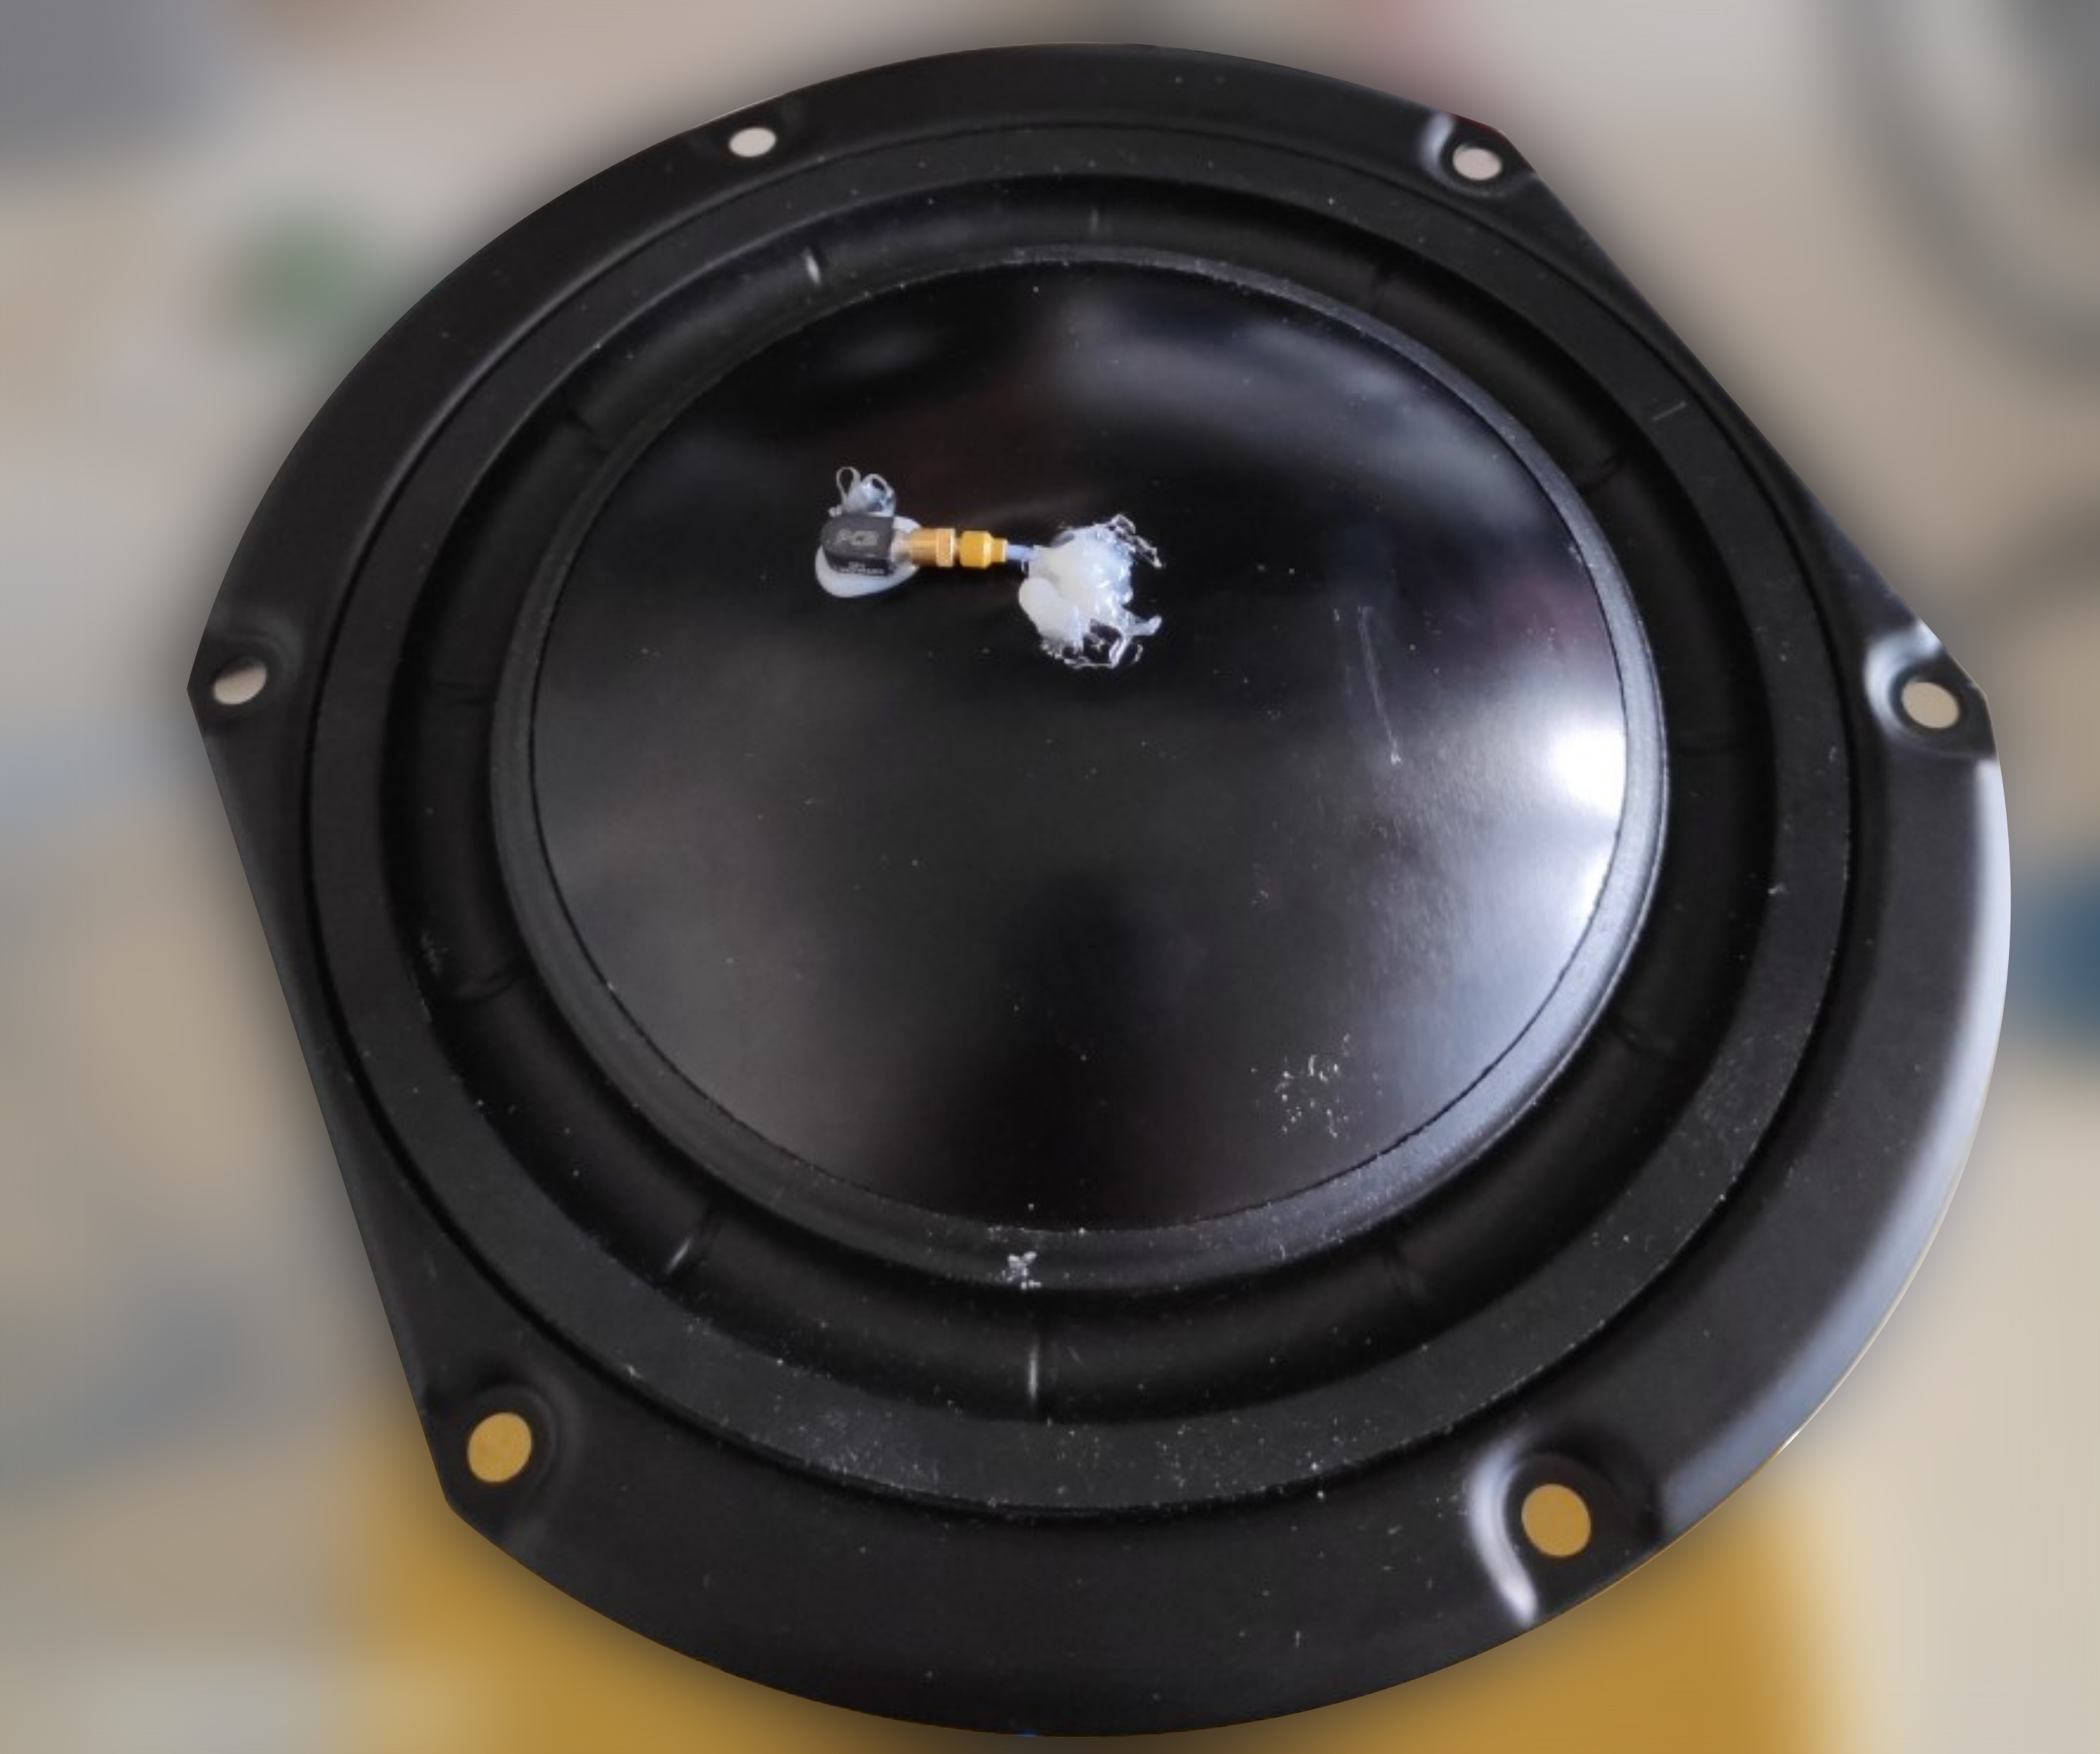
\includegraphics[width=.7\textwidth]{../fig/fig_InstrumentationHP/HPPeerless_WithAcc.png}};}
    \caption{Source acoustique secondaire avec l'accéléromètre collé sur sa membrane.}
    \label{fig:HPPeerless_WithAcc}
\end{figure}

\section{Vérification}
\subsection{Banc de mesures}

\subsection{Résultats}